\documentclass[tikz,border=8pt]{standalone}
\usepackage{tikz}
\usetikzlibrary{shapes.geometric,arrows.meta,positioning,calc}

\begin{document}
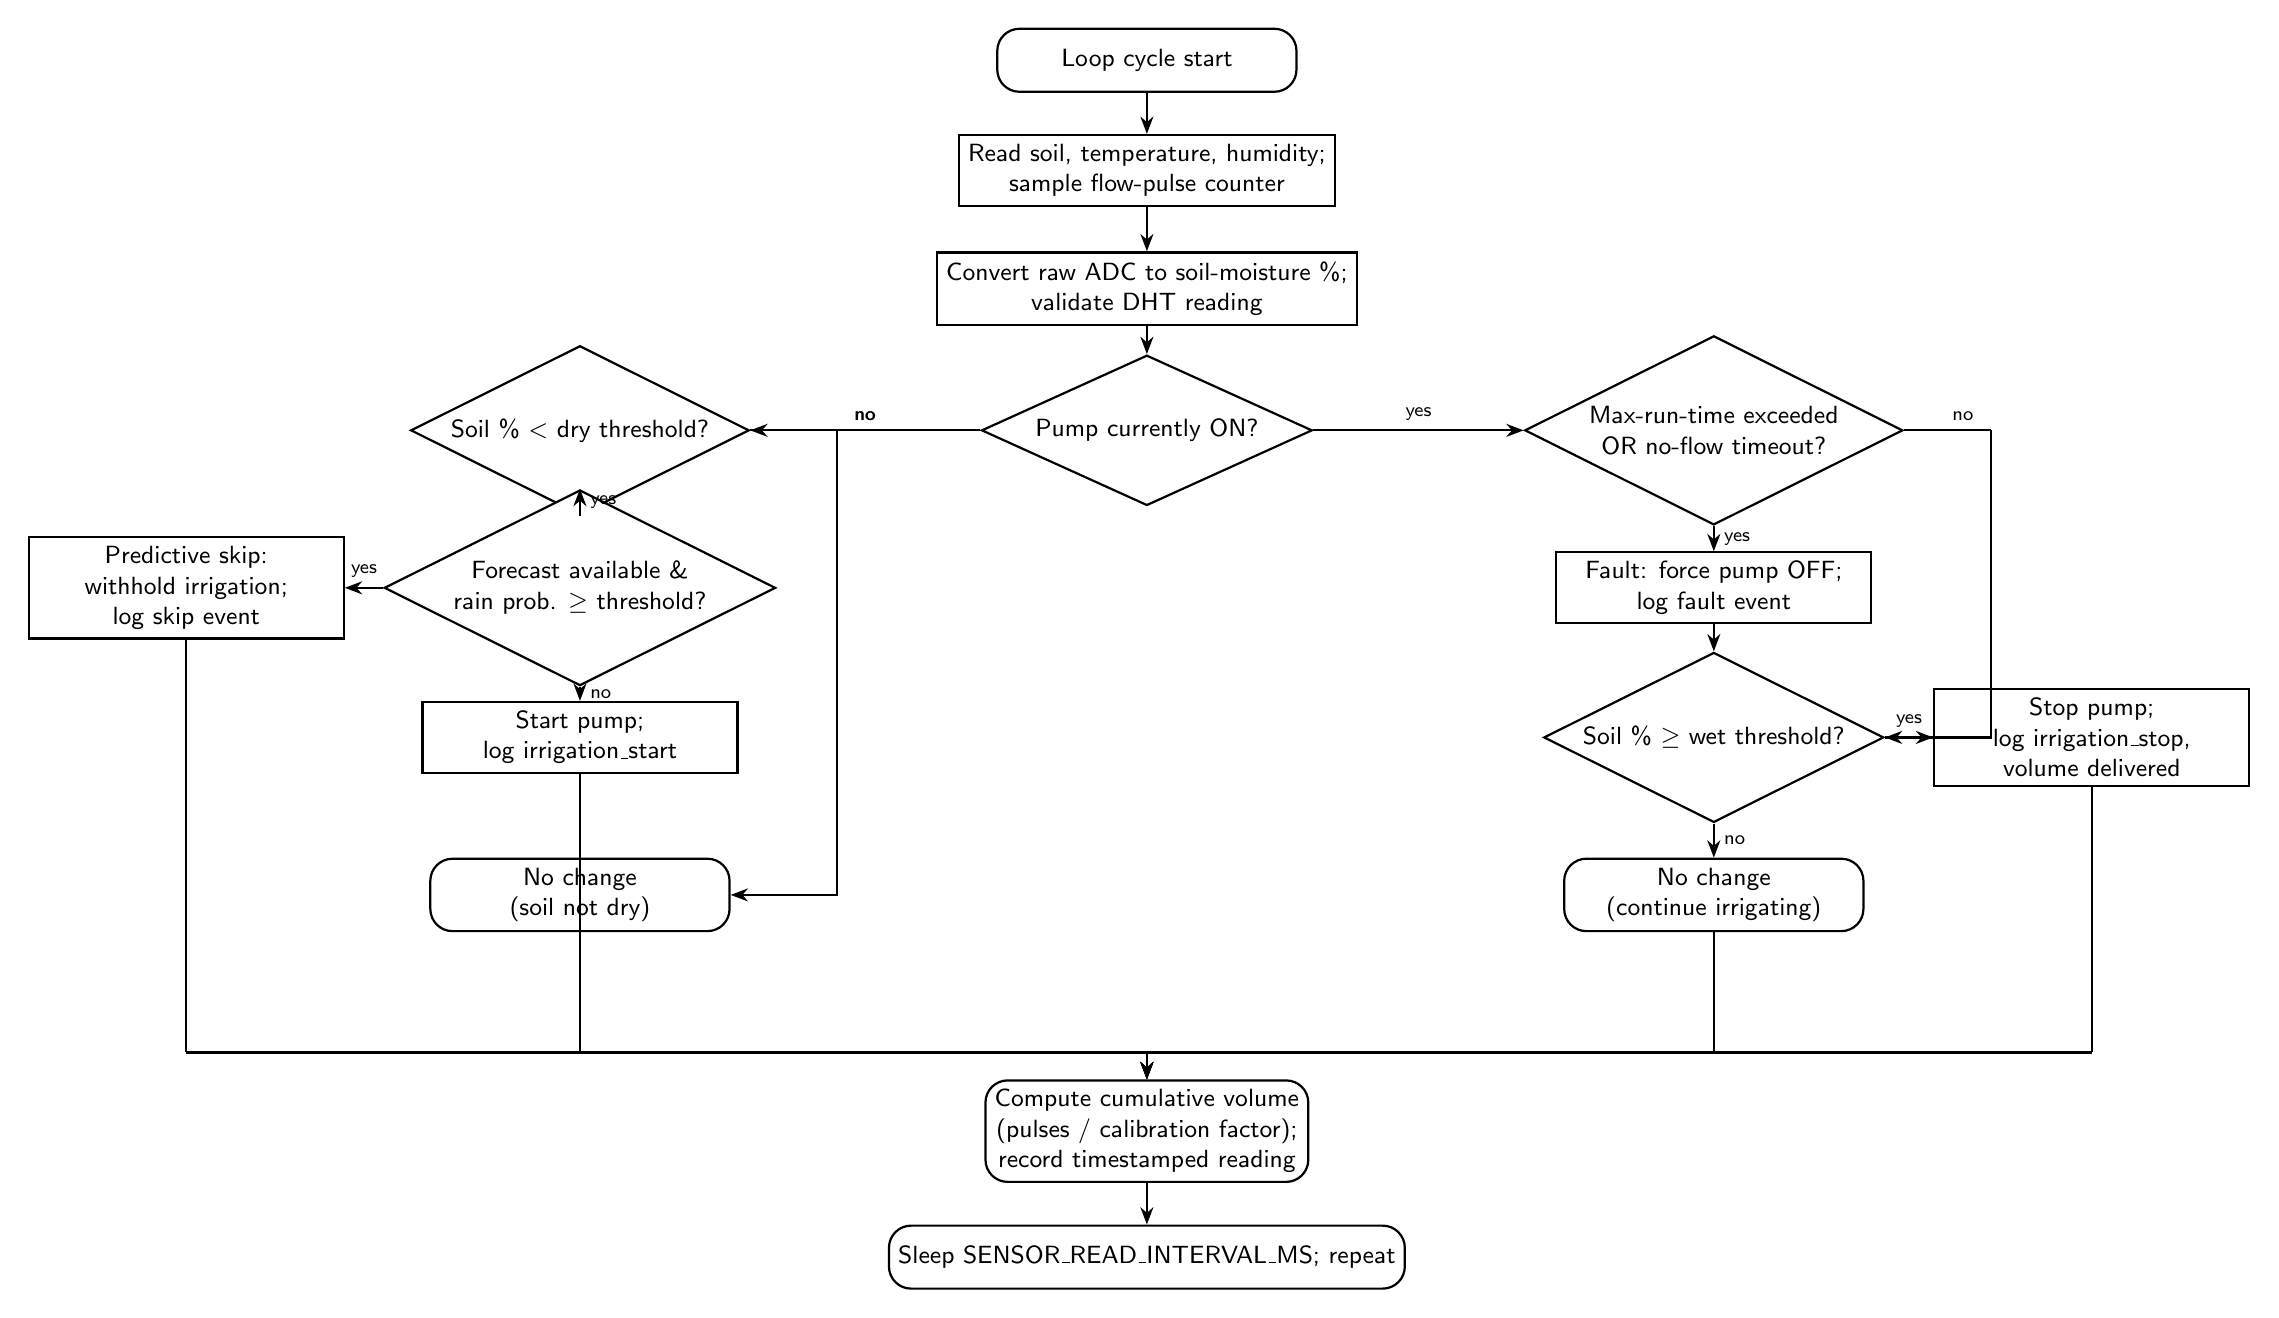
\begin{tikzpicture}[
  font=\sffamily\small,
  proc/.style={draw, thick, rectangle, minimum width=4.0cm, minimum height=0.9cm, align=center, fill=white},
  dec/.style={draw, thick, diamond, aspect=2.0, minimum width=4.2cm, minimum height=1.4cm, align=center, fill=white, inner sep=2pt},
  term/.style={draw, thick, rounded corners=8pt, minimum width=3.8cm, minimum height=0.8cm, align=center, fill=white},
  small/.style={font=\sffamily\scriptsize},
  arr/.style={-{Stealth[length=2.2mm]}, thick},
]

% ================= Shared spine (top) =================
\node[term] (start)   at (0,9.6)  {Loop cycle start};
\node[proc] (read)    at (0,8.2)  {Read soil, temperature, humidity;\\sample flow-pulse counter};
\node[proc] (convert) at (0,6.7)  {Convert raw ADC to soil-moisture \%;\\validate DHT reading};
\node[dec]  (pumpon)  at (0,4.9)  {Pump currently ON?};

\draw[arr] (start) -- (read);
\draw[arr] (read) -- (convert);
\draw[arr] (convert) -- (pumpon);

% ================= RIGHT branch: pump was ON =================
\node[dec]  (fault)     at (7.2,4.9)  {Max-run-time exceeded\\OR no-flow timeout?};
\node[proc] (faultstop) at (7.2,2.9)  {Fault: force pump OFF;\\log fault event};
\node[dec]  (wet)       at (7.2,1.0)  {Soil \% $\geq$ wet threshold?};
\node[proc] (stopon)    at (12.0,1.0) {Stop pump;\\log irrigation\_stop,\\volume delivered};
\node[term] (keepon)    at (7.2,-1.0) {No change\\(continue irrigating)};

\draw[arr] (pumpon.east) -- node[above,small]{yes} (fault.west);
\draw[arr] (fault.south) -- node[right,small]{yes} (faultstop.north);
\draw[arr] (faultstop.south) -- (wet.north);
\draw[thick] (fault.east) -- ++(1.1,0) coordinate (faultbypass);
\draw[arr]  (faultbypass) node[above,small,xshift=-10pt]{no} -- (faultbypass |- wet.east) -- (wet.east);
\draw[arr] (wet.east) -- node[above,small]{yes} (stopon.west);
\draw[arr] (wet.south) -- node[right,small]{no} (keepon.north);

% ================= LEFT branch: pump was OFF =================
\node[dec]  (dry)   at (-7.2,4.9)  {Soil \% $<$ dry threshold?};
\node[dec]  (rain)  at (-7.2,2.9)  {Forecast available \&\\rain prob. $\geq$ threshold?};
\node[proc] (skip)  at (-12.2,2.9) {Predictive skip:\\withhold irrigation;\\log skip event};
\node[proc] (starton) at (-7.2,1.0) {Start pump;\\log irrigation\_start};
\node[term] (nodecision) at (-7.2,-1.0) {No change\\(soil not dry)};

\draw[arr] (pumpon.west) -- node[above,small]{no} (dry.east);
\draw[thick] (dry.east) -- ++(1.1,0) coordinate (drybypass);
\draw[arr]  (drybypass) node[above,small,xshift=10pt]{no} -- (drybypass |- nodecision.east) -- (nodecision.east);
\draw[arr] (dry.south) -- node[right,small]{yes} (rain.north);
\draw[arr] (rain.west) -- node[above,small]{yes} (skip.east);
\draw[arr] (rain.south) -- node[right,small]{no} (starton.north);

% ================= Merge: all outcomes converge on logging =================
\node[term] (logall) at (0,-4.0) {Compute cumulative volume\\(pulses / calibration factor);\\record timestamped reading};

\def\collect{-3.0}
\draw[thick] (skip.south)       -- (skip.south |- 0,\collect);
\draw[thick] (starton.south)    -- (starton.south |- 0,\collect);
\draw[thick] (nodecision.south) -- (nodecision.south |- 0,\collect);
\draw[thick] (keepon.south)     -- (keepon.south |- 0,\collect);
\draw[thick] (stopon.south)     -- (stopon.south |- 0,\collect);
\draw[arr] (skip.south |- 0,\collect)       -- (0,\collect) -- (logall.north);
\draw[arr] (starton.south |- 0,\collect)    -- (0,\collect) -- (logall.north);
\draw[arr] (nodecision.south |- 0,\collect) -- (0,\collect) -- (logall.north);
\draw[arr] (keepon.south |- 0,\collect)     -- (0,\collect) -- (logall.north);
\draw[arr] (stopon.south |- 0,\collect)     -- (0,\collect) -- (logall.north);

\node[term] (endloop) at (0,-5.6) {Sleep SENSOR\_READ\_INTERVAL\_MS; repeat};
\draw[arr] (logall) -- (endloop);

\end{tikzpicture}
\end{document}
